\documentclass[letterpaper, 10 pt, conference]{sty/ieeeconf}

\IEEEoverridecommandlockouts

\overrideIEEEmargins

\usepackage{graphics}
\usepackage{epsfig}
\usepackage{amsmath}
\usepackage{amssymb}
\usepackage{txfonts}
\usepackage{tikz}
\usepackage[T1]{fontenc}

\DeclareMathOperator*{\argmax}{arg\,max}
\DeclareMathOperator*{\argmin}{arg\,min}

\begin{document}

\title{\LARGE \bf
Curbs Detection for a Pedestrian Robot
}

\author{
\authorblockN{
J\'{e}r\^{o}me Maye,
Ralf Kaestner,
and Roland Siegwart}
\authorblockA{
Autonomous Systems Lab, ETH Zurich, Switzerland\\
email: \{jerome.maye, ralf.kaestner, roland.siegwart\}@mavt.ethz.ch}
}

\maketitle

\begin{abstract}
This paper presents a novel ...

\end{abstract}

\section{Introduction}
CONTEXT OF THE PAPER.

SUMMARY OF THE PAPER.

CONTRIBUTIONS.

The rest of the paper is organized as follows. Section~\ref{sec:related}
summarizes the previous works related to ours. Section~\ref{sec:formulation}
introduces our Bayesian framework. Section~\ref{sec:exp} presents experimental
results. Section~\ref{sec:conc} outlines our conclusions and provides some
insights for future work.


\section{Related Work\label{sec:related}}
Some related works~\cite{oniga10polynomial,wijesoma04road,shin10drivable,pradeep08piece,yuan05dynamic,siegemund10curb}.


\section{Model\label{sec:model}}
In this Section, we establish the preliminary notations and introduce the
mathematical models that will be used throughout the paper.

\subsection{Measurements Representation}
A nodding laser range-finder produces scan measurements $\mathbf{s}_i=[r_i,
\theta_i,\psi_i]^\text{T}$ that are transformed into their corresponding
Cartesian 3D coordinates $\mathbf{p}_i=[x_i,y_i,z_i]^\text{T}$, where $r_i$ is
a range measurement, $\theta_i$ a pitch angle, and $\psi_i$ a bearing angle. The
sensing device has an error model which is typically a function of
$\mathbf{s}_i$, i.e. $e(\mathbf{s}_i)$. From a complete laser sweep, we obtain a
point cloud representation $\mathcal{P}=\{\mathbf{p}_1,\mathbf{p}_2,\dots,
\mathbf{p}_N\}$. $\mathcal{P}$ is finally projected onto a 2D grid $\mathcal{G}=
\{\mathcal{C}_1,\mathcal{C}_2,\dots,\mathcal{C}_M\}$, with cells $\mathcal{C}_i=
\{\mathbf{c}_i,h_i,l_i,\mathcal{I}_i\}$, where $\mathbf{c}_i$ is the center of
the cell, $h_i$ its height distribution, $l_i$ its label distribution, and
$\mathcal{I}_i=\{\mathbf{p}_j\mid\mathbf{p}_j\in\mathcal{P},j=\argmin_{j'}||
\mathbf{p}_{j'}-\mathbf{c}_i||,\mathbf{p}_{j_x}<\tau_{x_{max}},\mathbf{p}_{j_x}>
\tau_{x_{min}},\mathbf{p}_{j_y}<\tau_{y_{max}},\mathbf{p}_{j_y}>\tau_{y_{min}},
\mathbf{p}_{j_z}<\tau_{z_{max}},\mathbf{p}_{j_z}>\tau_{z_{min}}\}$. The
$\tau_{[x,y,z]_{[min,max]}}$ define boundaries for the 3D points.

The posterior height distribution is a normal distribution, such that $p(h_i)=
\mathcal{N}(h_i\mid\mu_{h_i},\sigma^2_{h_i},\mathcal{I}_i)$. $\mu_{h_i}$ is the
Maximum-Likelihood Estimate (MLE) for the cell mean computed with the values
$\mathbf{p}_{j_z}$, where $\mathbf{p}_j\in\mathcal{I}_i$. $\sigma^2_{h_i}$ is
the Maximum A-Posteriori (MAP) estimate for the cell variance. The prior
distribution for $\sigma^2_{h_i}$ is an inverse gamma distribution, where we
have inserted a simplified cell error model in the hyperparameters. The label
distribution is a discrete distribution over a set of labels
$\mathcal{L}=\{1,2,\dots,M\}$.

The grid $\mathcal{G}$ will also be referred to as a Digital Elevation Map (DEM)
in the rest of the paper. The choice of a DEM representation is mainly guided by
the final outcome of the algorithm, i.e. a traversability map for the planning
process. It is also convenient for defining Regions of Interest (ROI) in
$\mathcal{P}$ and for simplifying the subsequent computations. Whenever the
number of points that fall into a cell $\mathcal{C}_i$ is below a threshold,
i.e. $|\mathcal{I}_i|<\tau_{\mathcal{I}}$, it is flagged as invalid.

\subsection{Environment Model and Inference Task}
We assume a piecewise planar environment, i.e., the observed scene is composed
of a set of plane segments. Boundaries between plane segments define local
heights discontinuities that we shall term \emph{curbs} from now on. The major
inference task therefore boils down to discovering those plane segments. To this
end, we model the environment as a \emph{mixture of linear regressions}, which
yields the following generative process for the height values:

\begin{equation}
\label{eqn:mixture}
h_i\sim p(h_i\mid\Theta)=\sum_{k=1}^K\pi_k\mathcal{N}(h_i\mid
\mathbf{w}_k^\text{T}\boldsymbol{\phi}(\mathbf{c}_i),\sigma^2_k),
\end{equation}

where $\Theta=\{\boldsymbol{\pi},\mathbf{W},\boldsymbol{\sigma}^2\}$ is the set
of adaptive parameters, $\boldsymbol{\pi}=\{\pi_k\}$ are the mixture weights,
$\mathbf{W}=\{\mathbf{w}_k\}$ the regression coefficients,
$\boldsymbol{\sigma}^2=\{\sigma^2_k\}$ the regression variances, and
$\boldsymbol{\phi}(\mathbf{c}_i)=[1,\mathbf{c}_i]^\text{T}$ is the basis
function.

Similarly to Gaussian Mixture Models (GMM), one can resort to the popular
Expectation-Maximization (EM) algorithm~\cite{dempster77maximum} for estimating
the parameter set $\Theta$ given a set of observations
$\{\{h_i,\mathbf{c}_i\}\}_{i=1}^M$. The algorithm alternates between the
computation of \emph{responsibilities} $\gamma_{ik}$ given an old estimate
$\Theta^\text{old}$, and the computation of $\Theta^\text{new}$ given
$\Theta^\text{old}$ and $\gamma_{ik}$.

In order to determine the number of planes $k$ and the initial responsibilities,
we apply the algorithm presented in Section~\ref{sec:initial}. The following
responsibilities are then evaluated with the Conditional Random Field (CRF) of
Section~\ref{sec:crf} and the parameter set $\Theta^\text{new}$ with the method
of Section~\ref{sec:plane}.


\section{Initial Labeling\label{sec:initial}}
Our algorithm needs an initial rough estimate of the plane segments. This
initial estimate consists in labeling the DEM cells that belong to the same
plane segments. More formally, we refine our definition of plane segments to
$\mathcal{S}_i=\{\mathcal{C}_j\mid l_j=i\}$.

We use the graph-based algorithm from Felzenzswalb and
Huttenlocher~\cite{felzenszwalb04efficient}. Although this method was originally
designed for image segmentation, we can tune it for our purposes, image regions
corresponding to plane segments. We define an undirected graph
$\mathcal{G}=\{\mathcal{V},\mathcal{E}\}$, with vertices $v_i\in\mathcal{V}$ to
be segmented and edges $(v_i,v_j)\in\mathcal{E}$ for neighboring vertices. Each
edge has a weight $w((v_i,v_j))$ proportional to the dissimilarity between $v_i$
and $v_j$. In our particular setting, each grid cell $\mathcal{C}_i$ is aligned
with a vertex $v_i$ and each vertex has a 4-connected neighborhood. The goal of
the algorithm is to find a partition of $\mathcal{V}$ into components
$\mathcal{C}$ that correspond to the connected components of a graph
$\mathcal{G}'=\{\mathcal{V},\mathcal{E}'\}$, with
$\mathcal{E}'\subseteq\mathcal{E}$. We are interested in the partition such that
vertices in a component have a high similarity and vertices in different
components a low similarity. Therefore, edges between vertices in the same
component should have a low weight and edges between vertices in different
components a high weight. We define the weight function as the symmetric
Kullback-Leibler divergence between two cells, i.e.,
$w((v_i,v_j))=D_{KL}(h_i\mid\mid h_j)+D_{KL}(h_j\mid\mid h_i)$. For normal
distributions, the Kullback-Leibler divergence integrates analytically to
$D_{KL}(h_i\mid\mid h_j)=\frac{(\mu_i-\mu_j)^2}{2\sigma_j^2}+\frac{1}{2}
(\frac{\sigma_i^2}{\sigma_j^2}-1-\ln\frac{\sigma_i^2}{\sigma_j^2})$. The
algorithm starts with all vertices belonging to a different component. It then
iterates by merging components based on the comparison predicate

\begin{equation}
\label{eqn:comp_pred}
D(C_1,C_2) = \left\{
\begin{array}{l l}
\text{true} & \quad \text{if $Dif(C_1,C_2)>MInt(C_1,C_2)$ }\\
\text{false} & \quad \text{otherwise},
\end{array} \right.
\end{equation}

where $Dif(C_1,C_2)=\min w((v_i,v_j))$, $Int(C)=\max w(e)$,
$MInt(C_1,C_2)=\min(Int(C_1)+\tau(C_1),Int(C_2)+\tau(C_2))$ the minimum internal
difference, and $\tau(C)=k/|C|$. Two components should be disconnected if the
difference between them is large compared to the internal difference within at
least one of the components. $k$ is a scale parameter that controls the
preference for larger components. The algorithm runs in $O(m\log(m))$, where
$m$ is the number of edges in the graph and it is guaranteed to produce a
segmentation which is neither too fine nor too coarse.

The resulting segmentation defines a probability distribution $p(l_i^{(0)})$ for
each cell, with the domain of $l_i$ being the number of components. This initial
distribution is expressed as

\begin{equation}
\label{eqn:comp_pred}
p(l_i^{(0)}=j) = \left\{
\begin{array}{l l}
1 & \quad \text{if $C_i$ belongs to component $j$}\\
0 & \quad \text{otherwise}.
\end{array} \right.
\end{equation}


\section{Planes Estimation\label{sec:plane}}
In this Section, we will derive the necessary steps for updating the parameter
set $\Theta$. As we shall see, this will involve the responsibilities
$\gamma_{ik}$, i.e. $p(l_i=k)$, in a weighted linear regression framework.

According to standard literature on mixture models, we may compute the weight
$\pi_k$ of the k-th plane using the sum over cell responsibilities as follows
\begin{equation}
\label{eqn:weights}
\pi_k = \frac{1}{M'}\sum_{i=1}^{M'}\gamma_{ik},
\end{equation}

where once more $M'$ corresponds to the number of valid cells in the DEM.

The MLE of the other parameters are determined by maximizing the
\emph{complete-data} log likelihood, which is denoted by
$\log p(\mathbf{h}\mid\Theta)$ and $\mathbf{h}=[h_1,h_2,\dots,h_{M'}]^\text{T}$.

In order to estimate the regression coefficients $\mathbf{w}_k$ of the k-th
plane, we furthermore introduce the diagonal matrix
$\mathbf{R}_k=\text{diag}(\gamma_{ik})$ composed of the cell responsibilities.
We may then express the regression coefficients as a function of the
responsibilities and the so-called \emph{design matrix} $\boldsymbol{\Phi}=
[\boldsymbol{\phi}(\mathbf{c}_1), \boldsymbol{\phi}
(\mathbf{c}_2),\dots,\boldsymbol{\phi}(\mathbf{c}_{M'})]^\text{T}$:

\begin{equation}
\label{eqn:coeff}
\mathbf{w}_k = (\boldsymbol{\Phi}\mathbf{R}_k\boldsymbol{\Phi})^{-1}
\boldsymbol{\Phi}^\text{T}\mathbf{R}_k\mathbf{h}.
\end{equation}

In a final step, the regression variances are modified according to

\begin{equation}
\label{eqn:coeff}
\sigma^2_k = \frac{1}{M'}\sum_{i=1}^{M'} \gamma_{ik}(h_i-\mathbf{w}_k^\text{T}
\boldsymbol{\phi}(\mathbf{c}_i))^2.
\end{equation}

The attentive reader might notice that, apart from the introduction of
$\mathbf{R}_k$, these derivations are close to the case of the single linear
regression. Here, the responsibilities act as a weight to the computations, that
is, they control the degree of influence of a particular point to the
plane regression.


\section{Labeling with Conditional Random Field\label{sec:crf}}
Starting from the regression parameter set $\Theta$, we aim at computing the new
responsibilities $\gamma_{ik}$. In the classical mixture model framework, this
step is achieved by estimating

\begin{equation}
\label{eqn:responsibilities}
\gamma_{ik}\propto \pi_k\mathcal{N}(h_i\mid\mathbf{w}_k^\text{T}
\boldsymbol{\phi}(\mathbf{c}_i),\sigma^2_k).
\end{equation}

However, in our approach, we take the assumption that neighboring cells are more
likely to share the same label distribution, i.e., to be in the same plane
segment. A Conditional Random Field (CRF)~\cite{lafferty01conditional}
can advantageously propagate this information at a global scale on the entire
DEM and thus act as a \emph{smoother}. The initial labeling method from
Section~\ref{sec:initial}, due to its inherent local nature, might indeed result
in an over-segmented graph, that can be conveniently refined by the CRF.
Furthermore, a CRF provides the clear and sought probabilistic outcome in terms
of the distributions $l_i$.

A CRF is a discriminative and undirected graphical model globally conditioned on
the observations. In our setting, we use the same graph structure
$\mathcal{G}=\{\mathcal{V},\mathcal{E}\}$ as in Section~\ref{sec:initial} and
the task of the CRF is to infer the label distributions $l_i$ for each node. The
conditional joint distribution of the CRF is expressed as

\begin{eqnarray}
\label{eqn:crf_joint}
p(\mathbf{l}\mid\mathbf{h},\Theta)\propto
\phantom{aaaaaaaaaaaaaaaaaaaaaaaaaaaaaaaaaa}\\ \nonumber
\exp\bigg(\sum_{v_i\in\mathcal{V}}
\varphi(h_i,l_i,\Theta)+\sum_{(v_i,v_j)\in\mathcal{E}}
\psi(h_i,h_j,l_i,l_j,\Theta)\bigg),
\end{eqnarray}

where $\mathbf{l}=[l_1,l_2,\dots,l_{M'}]^\text{T}$, $\varphi=
\lambda\,f(h_i,l_i,\Theta)$ and $\psi=\mu\,g(h_i,h_j,l_i,l_j,\Theta)$ are the
\emph{node potential} and the \emph{edge potential} respectively. The potential
functions are positively defined functions. Intuitively, the node potential
reflects the likelihood of $h_i$ being labeled $l_i$, and the edge potential the
joint likelihood of $h_i$ and $h_j$ being labeled $l_i$ and $l_j$. In the
original formulation of CRF, the MLE of the weights $\lambda$ and $\mu$ are
learned from training data. Since we apply the CRF in an unsupervised manner, we
fix these weights empirically.

According to the above suggestions, we define the feature function as

\begin{equation}
\label{eqn:feature_function}
f(h_i,l_i=k,\Theta)=\pi_k\mathcal{N}(h_i\mid\mathbf{w}_k^\text{T}
\boldsymbol{\phi}(\mathbf{c}_i), \sigma^2_{h_i} + \sigma^2_k).
\end{equation}

In Equ.~\eqref{eqn:feature_function}, we note that the CRF does not required a
normalized feature function. Moreover, we have taken into account the
measurement noise by adding up the two variances $\sigma^2_{h_i}$ and
$\sigma^2_{k}$.

The edge function is finally defined by means of sigmoid functions as

\begin{eqnarray}
\label{eqn:edge_function}
g(h_i,h_j,l_i=k,l_j=l,\Theta)=\phantom{aaaaaaaaaaaaaaaaaaaaaaa}\\ \nonumber
\left\{
\begin{array}{l l}
1-(1+\exp(\sigma^2_{ij}-d_{ij}))^{-1} & \quad
\text{if $k=l$}\\
(1+\exp(\sigma^2_{ij}-d_{ij}))^{-1} & \quad
\text{otherwise},
\end{array} \right.
\end{eqnarray}

where $d_{ij}=|h_i-h_j|$ is the heights difference and $\sigma^2_{ij}=\sigma^2_i
+\sigma^2_j$ the sum of the measurement variances. The two sigmoid functions
intersect when $|h_i-h_j|=\sigma^2_i+\sigma^2_j$.

Once the node and edge potential functions are defined, we can perform inference
on the CRF. In our configuration, \emph{Loopy} Belief
Propagation (LBP)~\cite{weiss00correctness} is an appropriate approach. LBP is
an approximate message-passing algorithm that computes the marginal distribution
for each latent node $l_i$ conditioned on the observations $\mathbf{h}$. As
stated above, this distribution might play the role of responsibilities for the
mixture model.


\section{Experiments\label{sec:exp}}
In order to evaluate and validate the approach proposed in this paper, we have
conducted experiments on simulated and real-world data. Real-world data
has been acquired with a static nodding Laser Range-Finder (LRF) setup. Two
different lasers have been mounted, namely a SICK LMS-200 and an Hockuyo
UTM-30LX. We also tested our method on a pedestrian robot equipped with a
downward-facing SICK LMS-151 LRF that generates 3D point cloud while moving.

\subsection{Experimental Conditions and Quantitative Measures}

For the nodding lasers setup, we have recorded 33 3D point clouds with multiple
viewpoints from a standard street scene. For the pedestrian robot scenario, data
has been generated from a tour in a city center.

A quantitative evaluation of our algorithm can be carried out under various
inter-related perspectives: curb location in $x,y$, curb height in $z$,
number of planes, assignment of DEM cells to planes, plane parameters, or
computation time. Since we do not have a labeling of the curb position from
the dataset, we evaluate the predictive accuracy of a model trained
with one point cloud on another. To this end, we collect 19 point clouds from
the same position and perform cross-validation. Concretely, we iteratively
estimate the parameter set $\{\hat{\Theta},\mathbf{\hat{L}}\}$ using one point
cloud and evaluate the predictive error on the 18 remaining. The quantitative
measure is the Root Mean Square (RMS) error of prediction:

\begin{equation}
\label{eqn:rmspred}
RMSEP=\sqrt{\frac{1}{M}\sum_{i=1}^M(\hat{\mu}_{h_i}-\mathbf{\hat{w}}_k^\text{T}
\boldsymbol{\phi}(\mathbf{c}_i))^ 2)},
\end{equation}

where $M$ is the number of valid cells in the point cloud being predicted and
$\mathbf{\hat{w}}_k$ corresponds to the trained component at the MAP state of
the CRF at $\mathbf{c}_i$.

In order to further analyze our model, we have sampled point clouds from known
mixture of linear regression parameters and also evaluated in this case the RMS
error of the predicted parameters $\hat{\Theta}$ against their ground truth. In
the case of synthetic data, predicted curb location and height, and assignment
of cells to planes, can also be quantitatively evaluated. Furthermore, we can
judge the robustness and validity of our algorithm on various situations such
as T-junctions or inclined planes.

\subsection{Qualitative Evaluation}
Before we proceed with the actual quantitative analysis, we want to give a
glimpse on some qualitative results that demonstrate the pertinence of our
approach.

In Fig.~\ref{fig:europa}, our pedestrian robot navigates in a city center and
label curbs while driving. Since the point cloud is reconstructed while the
robot drives, curbs can only be detected behind the robot in this specific
situation. DEM patches are labeled sequentially and we achieve on-line and
real-time performance.

\begin{figure}[t]
\centering
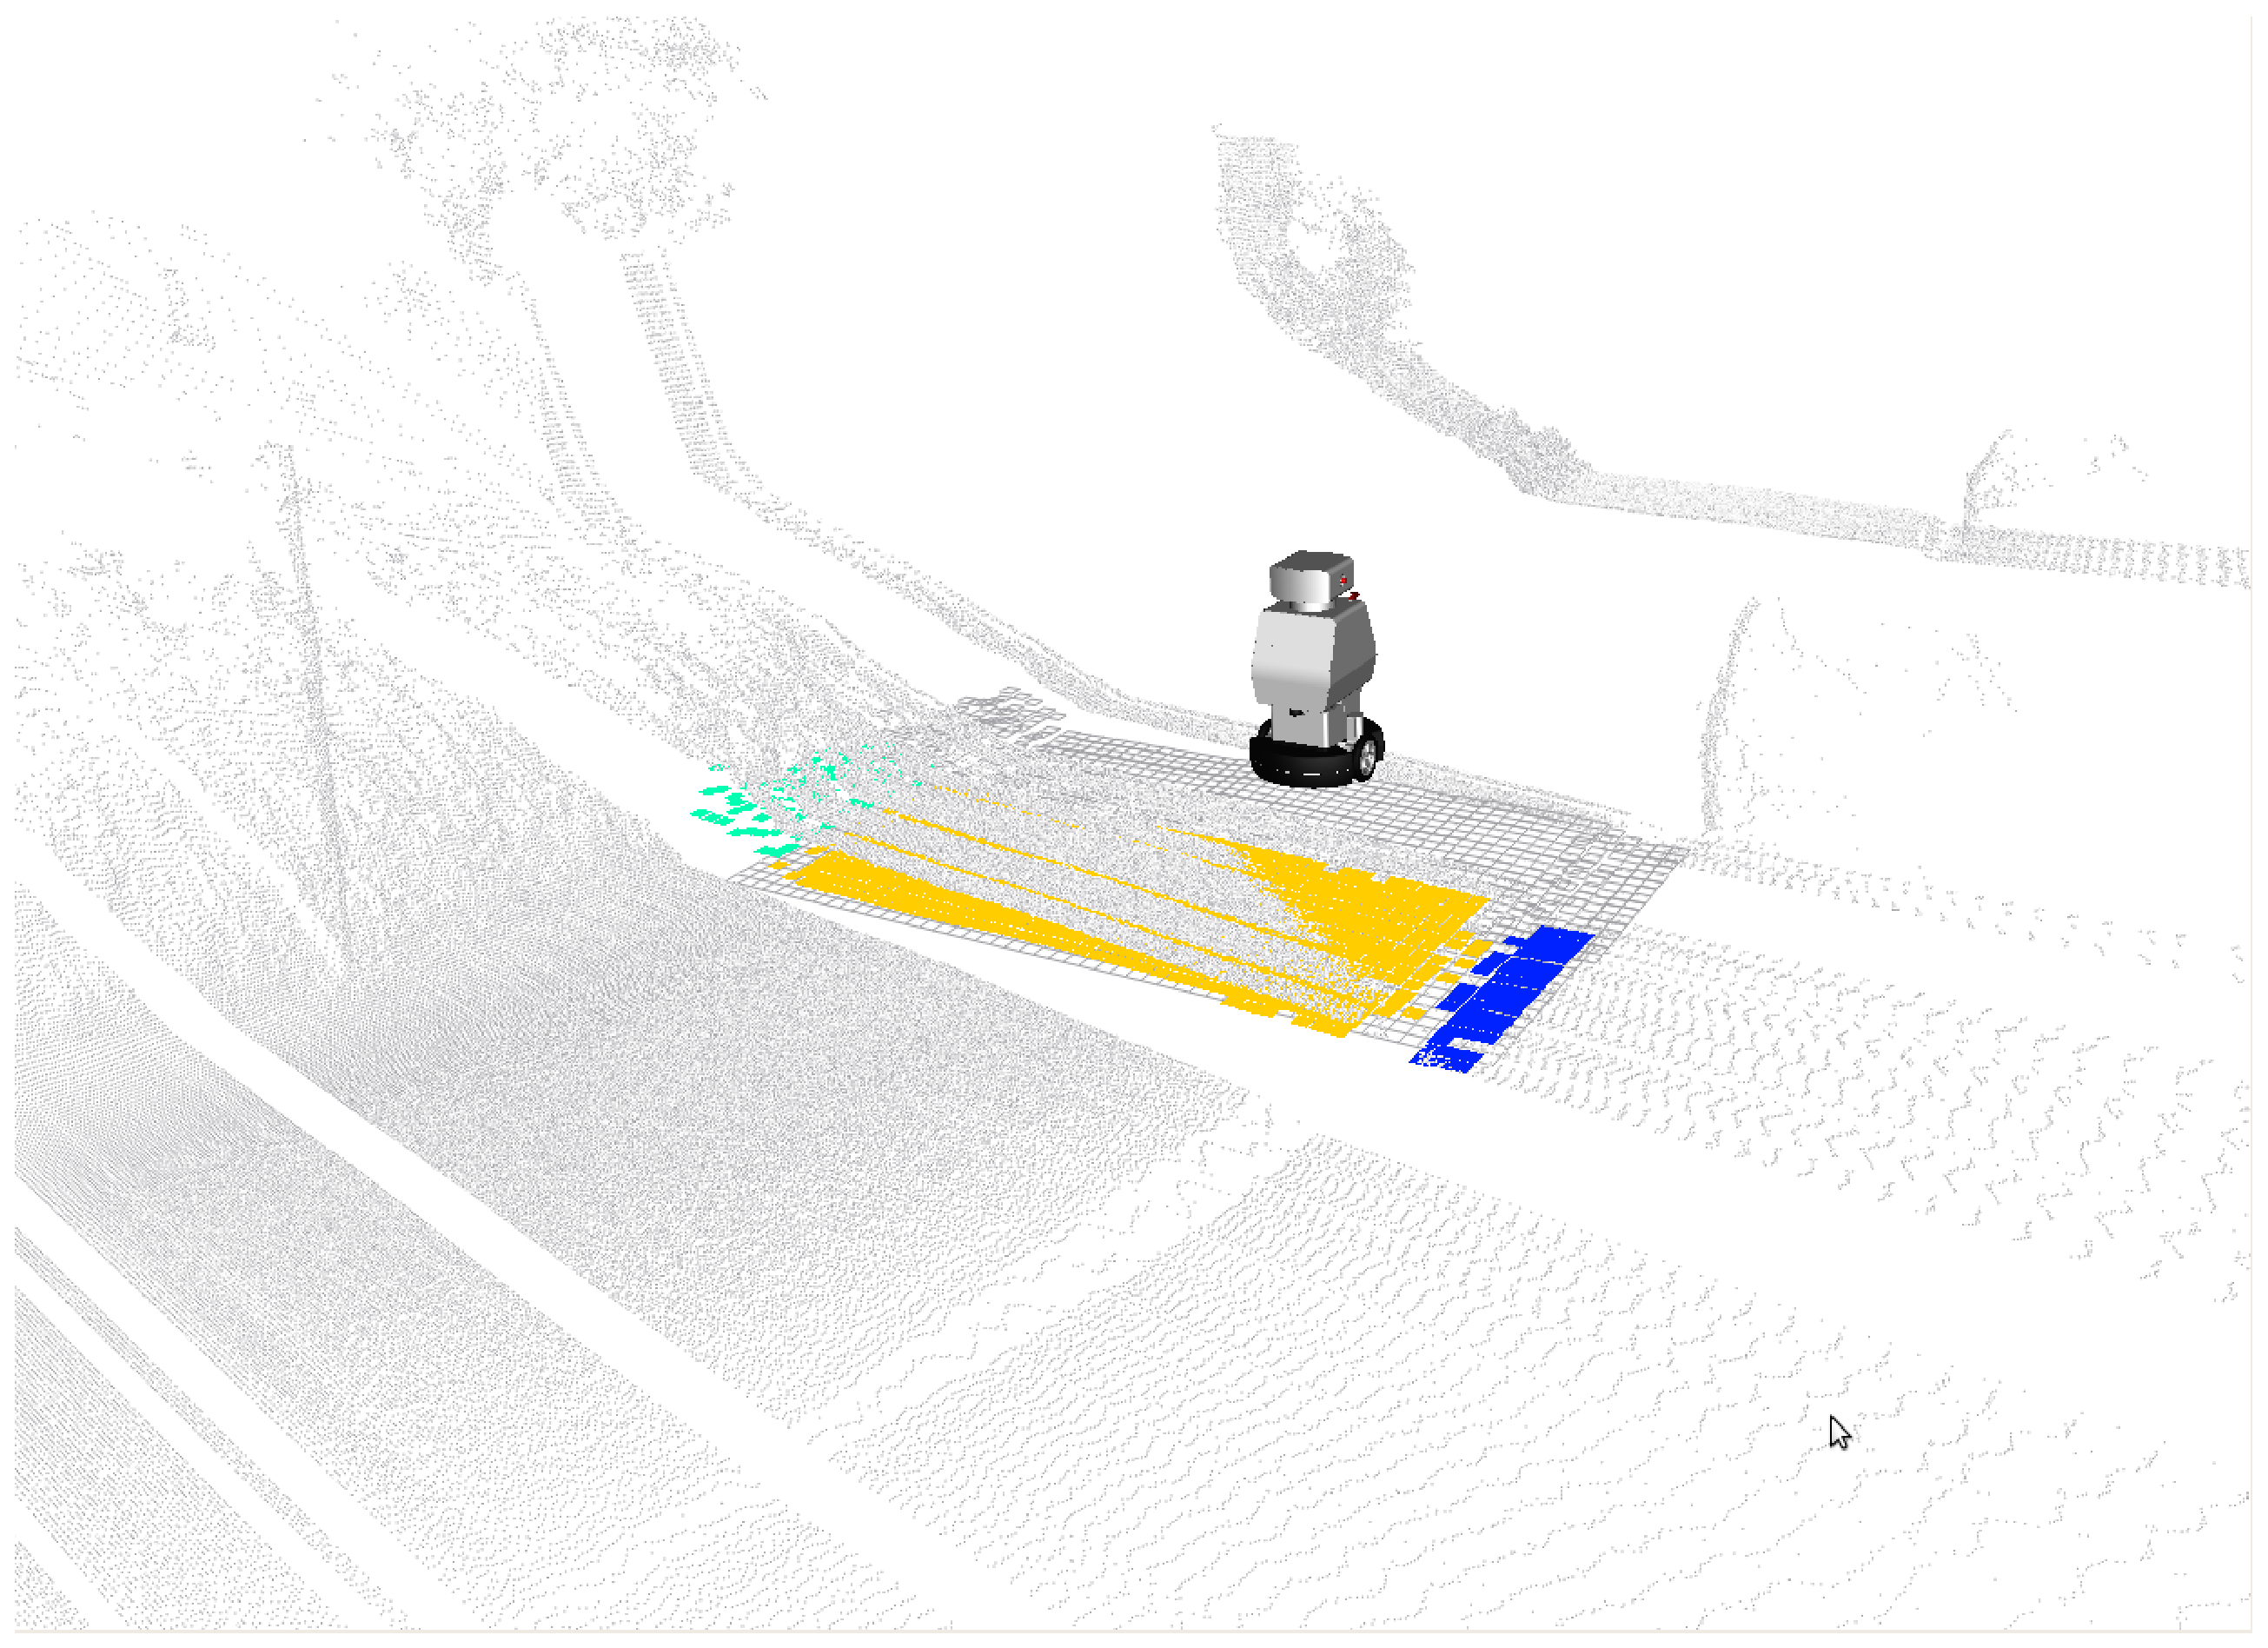
\includegraphics[width=\columnwidth]{fig/europa.eps}
\caption{Example of curb detection from a moving pedestrian robot. Colors
represent planes and curbs are located at their boundaries.}
\label{fig:europa}
\end{figure}

Fig.~\ref{fig:special} depicts a situation that a pedestrian robot might often
encounter when crossing a street. This experiment illustrates that our method
can cope with multiple viewpoints and environment configurations. Most of the
competitive approach would fail in this case.

\begin{figure}[t]
\centering
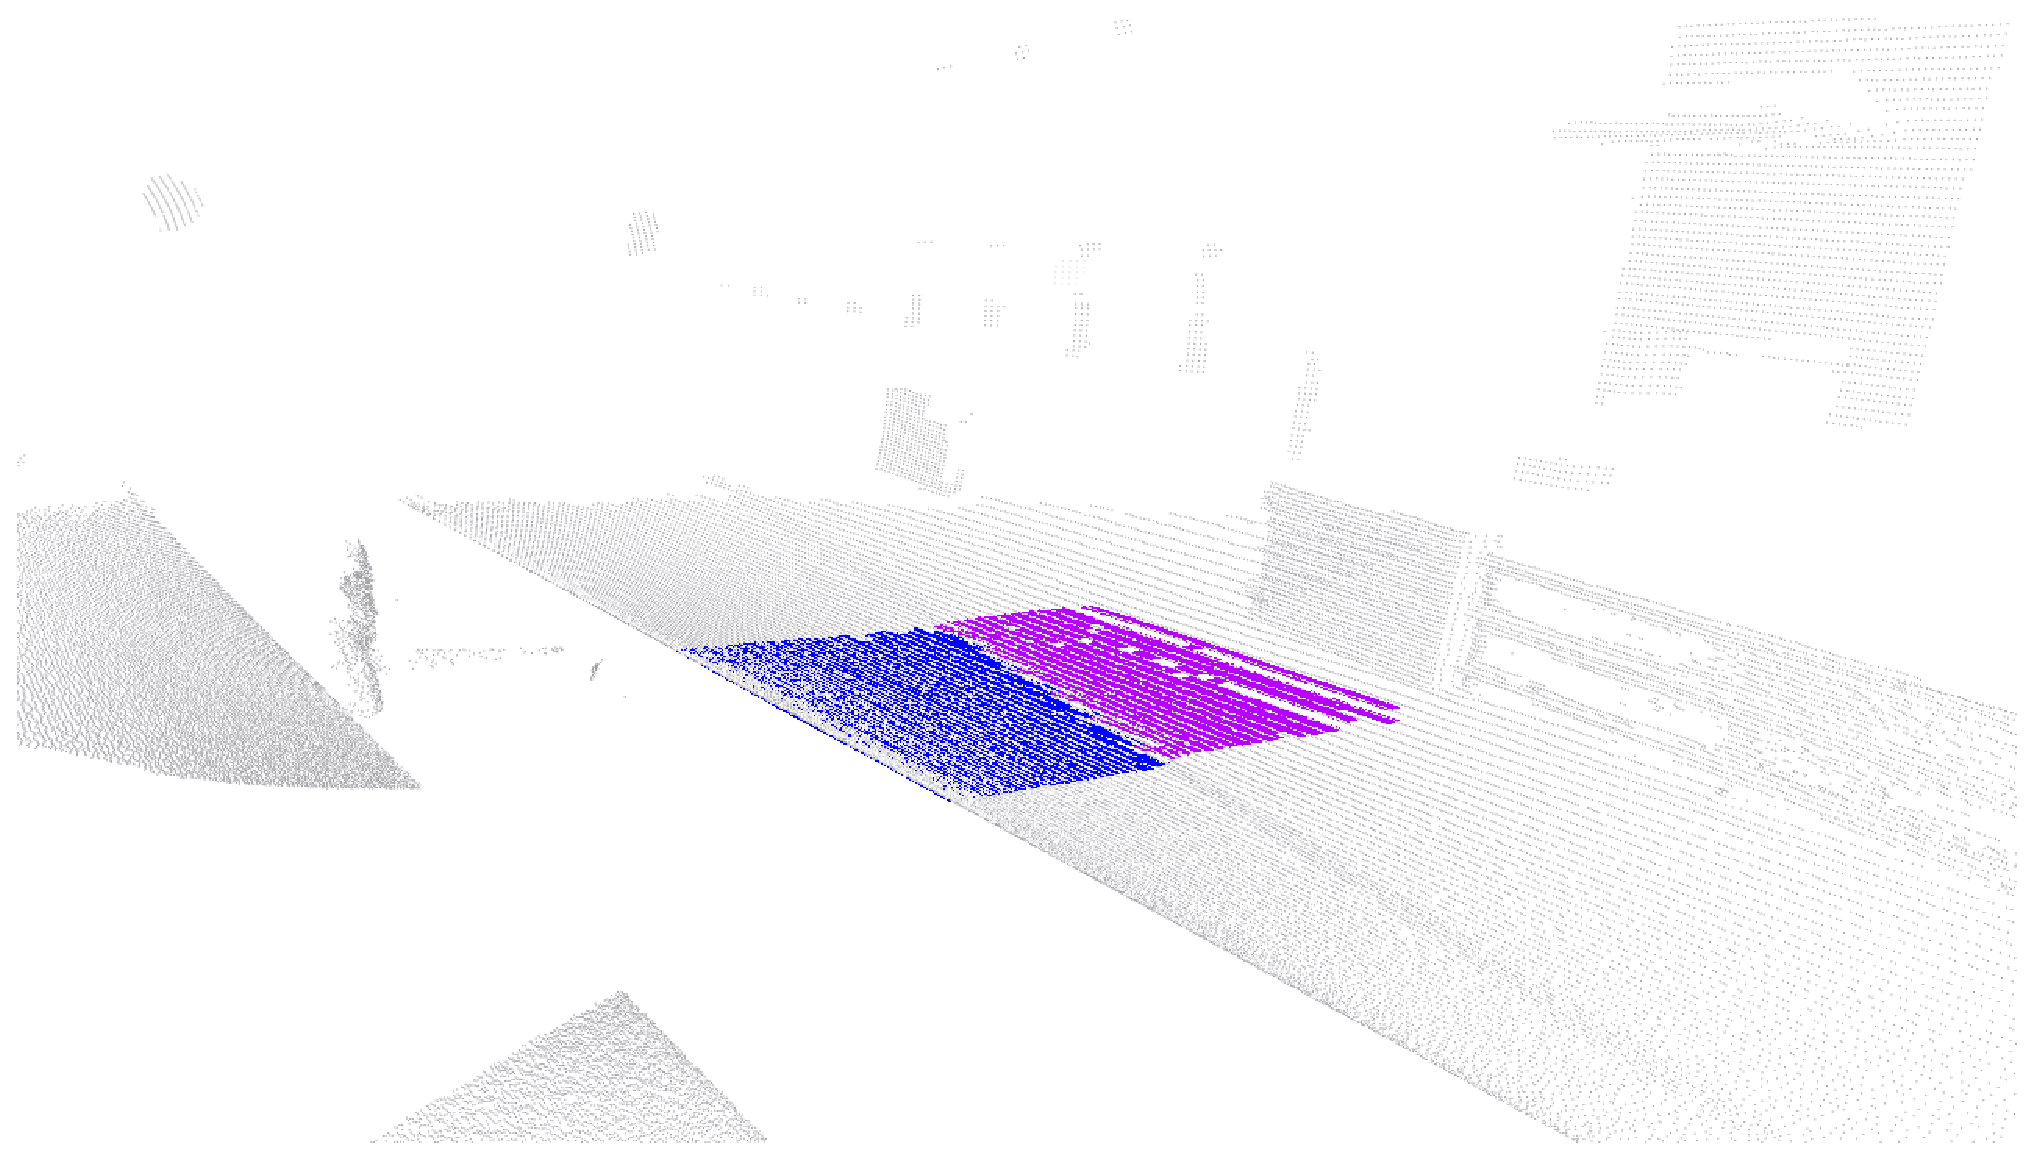
\includegraphics[width=\columnwidth]{fig/special.eps}
\caption{Example of curb detection in an unfavorable situation. Our algorithm
correctly label the planes, and thus curbs, under various viewpoints and
experimental settings.}
\label{fig:special}
\end{figure}

Fig.~\ref{fig:segment}

\subsection{Quantitative Evaluation and Discussion}



\section{Conclusion\label{sec:conc}}
In this paper, we have presented a novel approach for ...

In a further work, we aim at ...


\section*{Acknowledgment}
This work has partly been supported by the EC under FP7-231888-EUROPA.

\bibliographystyle{sty/IEEEtran}
\bibliography{bib/bibliography}

\end{document}
